\documentclass [11pt,twoside]{article}
%\usepackage[utf8]{inputenc}
\usepackage[T1]{fontenc}

%Page margins, header and footer positions
\usepackage{geometry}
 \geometry{
 a4paper,
 total={210mm,297mm},
 left=25mm,
 right=25mm,
 top=30mm,
 bottom=25mm,
 headsep=7mm}

\interfootnotelinepenalty=10000

%To display filling dots in the TOC for all entries
\usepackage[titles]{tocloft}
\renewcommand{\cftsecleader}{\cftdotfill{\cftdotsep}}

%Define new header and footer style
\usepackage{fancyhdr}

\pagestyle{fancy}
\fancyhf{}
\lhead{\color{Gray}{\small{Travlendar+ project by YOUR NAMES}}}
\lfoot{\textcolor{Gray}{\small{Copyright © 2017, YOUR NAMES – All rights reserved}}}
\rfoot{\textcolor{Gray}{\thepage}}
\renewcommand{\headrulewidth}{0pt}

%PACKAGES
\usepackage{wasysym}
\usepackage{pifont}

\newcommand{\supported}{\ding{52}\xspace}
\newcommand{\unsupported}{\ding{55}\xspace}
\newcommand{\partsupported}{\textcolor{black!40}{\ding{52}}\xspace}
\newcommand{\lowsupported}{\textcolor{black!20}{\ding{52}}\xspace}
\newcommand{\unknowsupported}{\textbf{?}\xspace}

%Font: Times
\usepackage{times}
%Change monospaced font
\renewcommand{\ttdefault}{lmtt}

%tables
\usepackage{tabu}
\usepackage{tabularx}
\usepackage{ltablex}
\usepackage{longtable}
\usepackage{float} % To allow the use of H modifier in long tables

%landscape mode
\usepackage{pdflscape}
\usepackage{rotating}
\usepackage{caption}

%make landscape mode be sensitive to even and odd pages
%start
\def\myrotate{\ifodd\c@page\else-\fi 90}
\makeatletter
\global\let\orig@begin@landscape=\landscape%
\global\let\orig@end@landscape=\endlandscape%
\gdef\@true{1}
\gdef\@false{0}
\gdef\landscape{%
    \global\let\within@landscape=\@true%
    \orig@begin@landscape%
}%
\gdef\endlandscape{%
    \orig@end@landscape%
    \global\let\within@landscape=\@false%
}%
\@ifpackageloaded{pdflscape}{%
    \gdef\pdf@landscape@rotate{\PLS@Rotate}%
}{
    \gdef\pdf@landscape@rotate#1{}%
}
\let\latex@outputpage\@outputpage
\def\@outputpage{
    \ifx\within@landscape\@true%
        \if@twoside%
            \ifodd\c@page%
                \gdef\LS@rot{\setbox\@outputbox\vbox{%
                    \pdf@landscape@rotate{-90}%
                    \hbox{\rotatebox{90}{\hbox{\rotatebox{180}{\box\@outputbox}}}}}%
                }%
            \else%
                \gdef\LS@rot{\setbox\@outputbox\vbox{%
                    \pdf@landscape@rotate{+90}%
                    \hbox{\rotatebox{90}{\hbox{\rotatebox{0}{\box\@outputbox}}}}}%
                }%
            \fi%
        \else%
            \gdef\LS@rot{\setbox\@outputbox\vbox{%
                \pdf@landscape@rotate{+90}%
                \hbox{\rotatebox{90}{\hbox{\rotatebox{0}{\box\@outputbox}}}}}%
            }%
        \fi%
    \fi%
    \latex@outputpage%
}
\makeatother
%end

%graphics
\usepackage{graphicx}
\usepackage[dvipsnames, table]{xcolor}
%If you upload images from PC, you need to insert code for the path here (different for Windows and Unix OS)

%References
%\usepackage{xpatch}
%\usepackage[backend=biber, style=numeric, citestyle=numeric, sorting=none]{biblatex}
%\addbibresource{main.bib}

%Other
\usepackage{ifthen}
\usepackage{xspace}
\usepackage{enumitem}
\usepackage{amssymb}
\usepackage[pdftex, colorlinks]{hyperref}
\newcommand{\comment}[1]{{\color{Red}$\blacktriangleright$ Comment: #1 $\blacktriangleleft$}}


% Some utilities\ldots
\usepackage{soul}
\usepackage{tikz}

\usetikzlibrary{calc}
\usetikzlibrary{decorations.pathmorphing}


\makeatletter

\newcommand{\defhighlighter}[3][]{%
  \tikzset{every highlighter/.style={color=#2, fill opacity=#3, #1}}%
}

\defhighlighter{yellow}{.5}

\newcommand{\highlight@DoHighlight}{
  \fill [ decoration = {random steps, amplitude=1pt, segment length=15pt}
        , outer sep = -15pt, inner sep = 0pt, decorate
       , every highlighter, this highlighter ]
        ($(begin highlight)+(0,8pt)$) rectangle ($(end highlight)+(0,-3pt)$) ;
}

\newcommand{\highlight@BeginHighlight}{
  \coordinate (begin highlight) at (0,0) ;
}

\newcommand{\highlight@EndHighlight}{
  \coordinate (end highlight) at (0,0) ;
}

\newdimen\highlight@previous
\newdimen\highlight@current

\DeclareRobustCommand*\highlight[1][]{%
  \tikzset{this highlighter/.style={#1}}%
  \SOUL@setup
  %
  \def\SOUL@preamble{%
    \begin{tikzpicture}[overlay, remember picture]
      \highlight@BeginHighlight
      \highlight@EndHighlight
    \end{tikzpicture}%
  }%
  %
  \def\SOUL@postamble{%
    \begin{tikzpicture}[overlay, remember picture]
      \highlight@EndHighlight
      \highlight@DoHighlight
    \end{tikzpicture}%
  }%
  %
  \def\SOUL@everyhyphen{%
    \discretionary{%
      \SOUL@setkern\SOUL@hyphkern
      \SOUL@sethyphenchar
      \tikz[overlay, remember picture] \highlight@EndHighlight ;%
    }{%
    }{%
      \SOUL@setkern\SOUL@charkern
    }%
  }%
  %
  \def\SOUL@everyexhyphen##1{%
    \SOUL@setkern\SOUL@hyphkern
    \hbox{##1}%
    \discretionary{%
      \tikz[overlay, remember picture] \highlight@EndHighlight ;%
    }{%
    }{%
      \SOUL@setkern\SOUL@charkern
    }%
  }%
  %
  \def\SOUL@everysyllable{%
    \begin{tikzpicture}[overlay, remember picture]
      \path let \p0 = (begin highlight), \p1 = (0,0) in \pgfextra
        \global\highlight@previous=\y0
        \global\highlight@current =\y1
      \endpgfextra (0,0) ;
      \ifdim\highlight@current < \highlight@previous
        \highlight@DoHighlight
        \highlight@BeginHighlight
      \fi
    \end{tikzpicture}%
    \the\SOUL@syllable
    \tikz[overlay, remember picture] \highlight@EndHighlight ;%
  }%
  \SOUL@
}

\makeatother

% Common abbrev. are set as commands to ensure proper spacing after the dot
\RequirePackage{xspace}
\newcommand{\ie}{i.e.\@\xspace}
\newcommand{\aka}{a.k.a.\@\xspace}
\newcommand{\Ie}{I.e.\@\xspace}
\newcommand{\cf}{cf.\@\xspace}
\newcommand{\Cf}{Cf.\@\xspace}
\newcommand{\eg}{e.g.\@\xspace}
\newcommand{\Eg}{E.g.\@\xspace}
\newcommand{\etal}{et al.\@\xspace}
\newcommand{\etc}{etc.\@\xspace}
\newcommand{\wrt}{w.r.t.\@\xspace}
\newcommand{\Wrt}{W.r.t.\@\xspace}



\date{}

%\documentclass[12pt]{article}
\usepackage[english]{babel}
\usepackage{natbib}
\usepackage{url}
\usepackage{ulem}

\usepackage[section]{placeins}
\usepackage[dvipsnames]{xcolor}
\usepackage{listings}
\usepackage{alloy-style}

\usepackage{graphicx}
\usepackage{subcaption}

%\usepackage[utf8x]{inputenc}
%\usepackage{amsmath}
%\usepackage{graphicx}
%\graphicspath{{images/}}
%\usepackage{parskip}
%\usepackage{fancyhdr}
%\usepackage{vmargin}
%\setmarginsrb{3 cm}{2.5 cm}{3 cm}{2.5 cm}{1 cm}{1.5 cm}{1 cm}{1.5 cm}

\title{TrackMe Requirement Analysis and Specification Document}								% Title
\author{Andrea Biscontini, Marco Gelli, Alvise de' Faveri Tron}								% Author
\date{11 Nov 2018}											% Date

\makeatletter
\let\thetitle\@title
\let\theauthor\@author
\let\thedate\@date
\makeatother

\pagestyle{fancy}
\fancyhf{}
\cfoot{\thepage}

\begin{document}
%TITLE PAGE

\title{2} 

%%%%%%%%%%%%%%%%%%%%%%%%%%%%%%%%%%%%%%%%%%%%%%%%%%%%%%%%%%%%%%%%%%%%%%%%%%%%%%%%%%%%%%%%%

\begin{titlepage}
	\centering
    \vspace*{0.5 cm}
    
\includegraphics[scale = 0.75]{LaTeX/Images/PolimiLogo.png}\\[1.0 cm]	% University Logo
    \textsc{\LARGE MSc in Computer Science and Engineering}\\[2.0 cm]	% University Name
	\textsc{\Large Software Engineering 2 Project}\\[0.5 cm]				% Course Code
	\rule{\linewidth}{0.2 mm} \\[0.4 cm]
	{ \huge \bfseries \thetitle}\\
	\rule{\linewidth}{0.2 mm} \\[1.5 cm]
	
	\begin{minipage}{0.4\textwidth}
		\begin{flushleft} \large
			\emph{Professor:}\\
			Elisabetta di Nitto\\
			\end{flushleft}
			\end{minipage}~
			\begin{minipage}{0.4\textwidth}
            
			\begin{flushright} \large
			\emph{Authors :} \\
			Andrea Biscontini - 901310\\
			Marco Gelli - 901470\\
			Alvise de'Faveri Tron - 920882\\
		\end{flushright}
        
	\end{minipage}\\[2 cm]
	
	
    
    
    
    
	
\end{titlepage}

%%%%%%%%%%%%%%%%%%%%%%%%%%%%%%%%%%%%%%%%%%%%%%%%%%%%%%%%%%%%%%%%%%%%%%%%%%%%%%%%%%%%%%%%%




\setcounter{page}{2}


%------------------------------------------------------------------------------------------------------------------------------------------------
\newpage
%\addcontentsline{toc}{section}{Table of Contents}
\tableofcontents
\newpage
%\addcontentsline{toc}{section}{List of Figures}
%\listoffigures
%\addcontentsline{toc}{section}{List of Tables}
%\listoftables

%------------------------------------------------------------------------------------------------------------------------------------------------
\clearpage
{\color{Blue}{\section{Introduction}}}
\label{sect:introduction}
prima dei sottocapitoli
\subsection{Purpose}
This document represent the Requirement Analysis and Specification Document of the Data4Help system. Here it's described the general purpose of the system, the functional and non-functional requirements that it must respect and the assumption through which we achieve all it's goal. This document is addressed to all the stakeholder of this system, which means final clients but also management, developer, testers and more.\\
The Data4Help system is composed by an user side smartphone Application and a web based query service for the third parties. The user-side App has the task to collect data from all the devices connected to the user's smartphone and send them to the TrackMe database. The web service is instead used by third parties to submit data request to TrackMe and, if they are successful, receive the most recent data collected on the proprietary databases.
AutomatedSOS is instead an user-side integration for the Data4Help service. Registered users' real time data are here monitored and, if there is any signal of possible health problems, local emergency numbers are called and an ambulance is called to intervene at the customer location.
Track4Run isanother ananotheranotheranotheranotherother system built upon Data4Help. Here users can become run organizers, enroll in scheduled runs and spectate live runs through a map with live GPS ranotheranotheranotherunners position.
\subsection{Scope}
\subsubsection{Description of the given problem}
As stated in the above section, Data4Help main goal is to collect user's data and made them available to third parties, all while guaranteeing the user privacy and consensus in personal data processing. To collect these data, the system needs to connect to users' smartwearables and download all the relevant produced data to TrackMe proprietary servers. Then this data are processed by TrackMe and whenever a request for data arrives from the third parties, if the request is successful, they're made available to them. Third parties could also desire to look for future changes in the data they requested, so an auxiliary subscription to new data is also made available at request time. Other than that, to simplify the data request procedure, this has been divided in two types of request: single user data request, that is forwarded directly to the individual that can accept or refuse it, and request for anonymized data of groups of individual, that is handled by TrackMe and it's always successful if there is the possibility to render the data anonym.
On top of the Data4Help system, that is used mainly by third party as a data retrieving service, there are AutomatedSOS and Track4Run. These service are instead to be used by an user of Data4Help. AutomatedSOS means is to help elderly or non-healty people to monitor their health status and intervene in the case of an emergency. In fact the goal of AutomatedSOS is to be very reactive (maximum 5 seconds) whenever a possible health problem is signaled and to immediately call emergency number and an ambulance for the location of the client.
Track4Run is instead a system designed for athletes and runners in which it's possible to organize, partecipate and spectate organized running competitions. Here any user can become the organizer of a run by creating one. The run creation procedure here is made really simple for the organizer, who needs only to insert the needed infos and select a route for the run on the map. When a run is created, every other user can enroll to it. To give an even better service, there is also the possibility to spectate a run on the App, which means follow every runner's position on a live GPS map.

The whole system ....
\subsubsection{Current System}
\subsubsection{Goals}
\begin{itemize}
\item \textbf{G1} Data4Help must be able to keep track of real time health status and position from registered users
\item \textbf{G2} Data4Help should allow third parties to gather information from a single user or from an anonymous group of users
\item \textbf{G3} Data4Help should allow third parties to subscribe to new data and receive them as soon as they're produced
\item \textbf{G4} AutomatedSOS should be able to identify an health emergency when the user data are below/exceeding a certain thresholds
\item \textbf{G5} AutomatedSOS must call an ambulance when it detects a health emergency
\item \textbf{G7} Track4Run allows a user to become an organizer of a run, so that he/she can create and manage a run
\item \textbf{G8} Track4Run allows a user to partecipate to an organized run
\item \textbf{G9} Track4Run allows a spectator to track the position of the partecipants of a run 
\end{itemize}
\subsection{Definitions, Acronyms, Abbreviations}
\subsubsection{Definitions}
third party, data source, synchronization, parameter, threshold,

\subsubsection{Acronyms}
\begin{itemize}
\item \textbf{RASD}: Requirement Analysis and Specification Document
\item \textbf{API}: Application Programming Interface
\item \textbf{GPS}: Global Positioning System
\item \textbf{GDPR}: General Data Protection Regulation
\end{itemize}

\subsubsection{Abbreviations}
\begin{itemize}
\item \textbf{D4H}: Data4Help
\item \textbf{ASOS}: AutomatedSOS
\item \textbf{T4R}: Track4Run
\item \textbf{Gn}: n-th goal
\item \textbf{Dn}: n-th domain assumption
\item \textbf{Rn}: n-th functional requirement
\end{itemize}
\subsection{Revision history}
quattro
\subsection{Reference Documents}
cinque
\subsection{Document Structure}
sei
%what you write here is a comment that is not shown in the final text

%------------------------------------------------------------------------------------------------------------------------------------------------
\clearpage
{\color{Blue}{\section{Overall Description}}}
\label{sect:overview}
Here you can see how to include an image in your document.

\begin{sidewaysfigure}
\centering
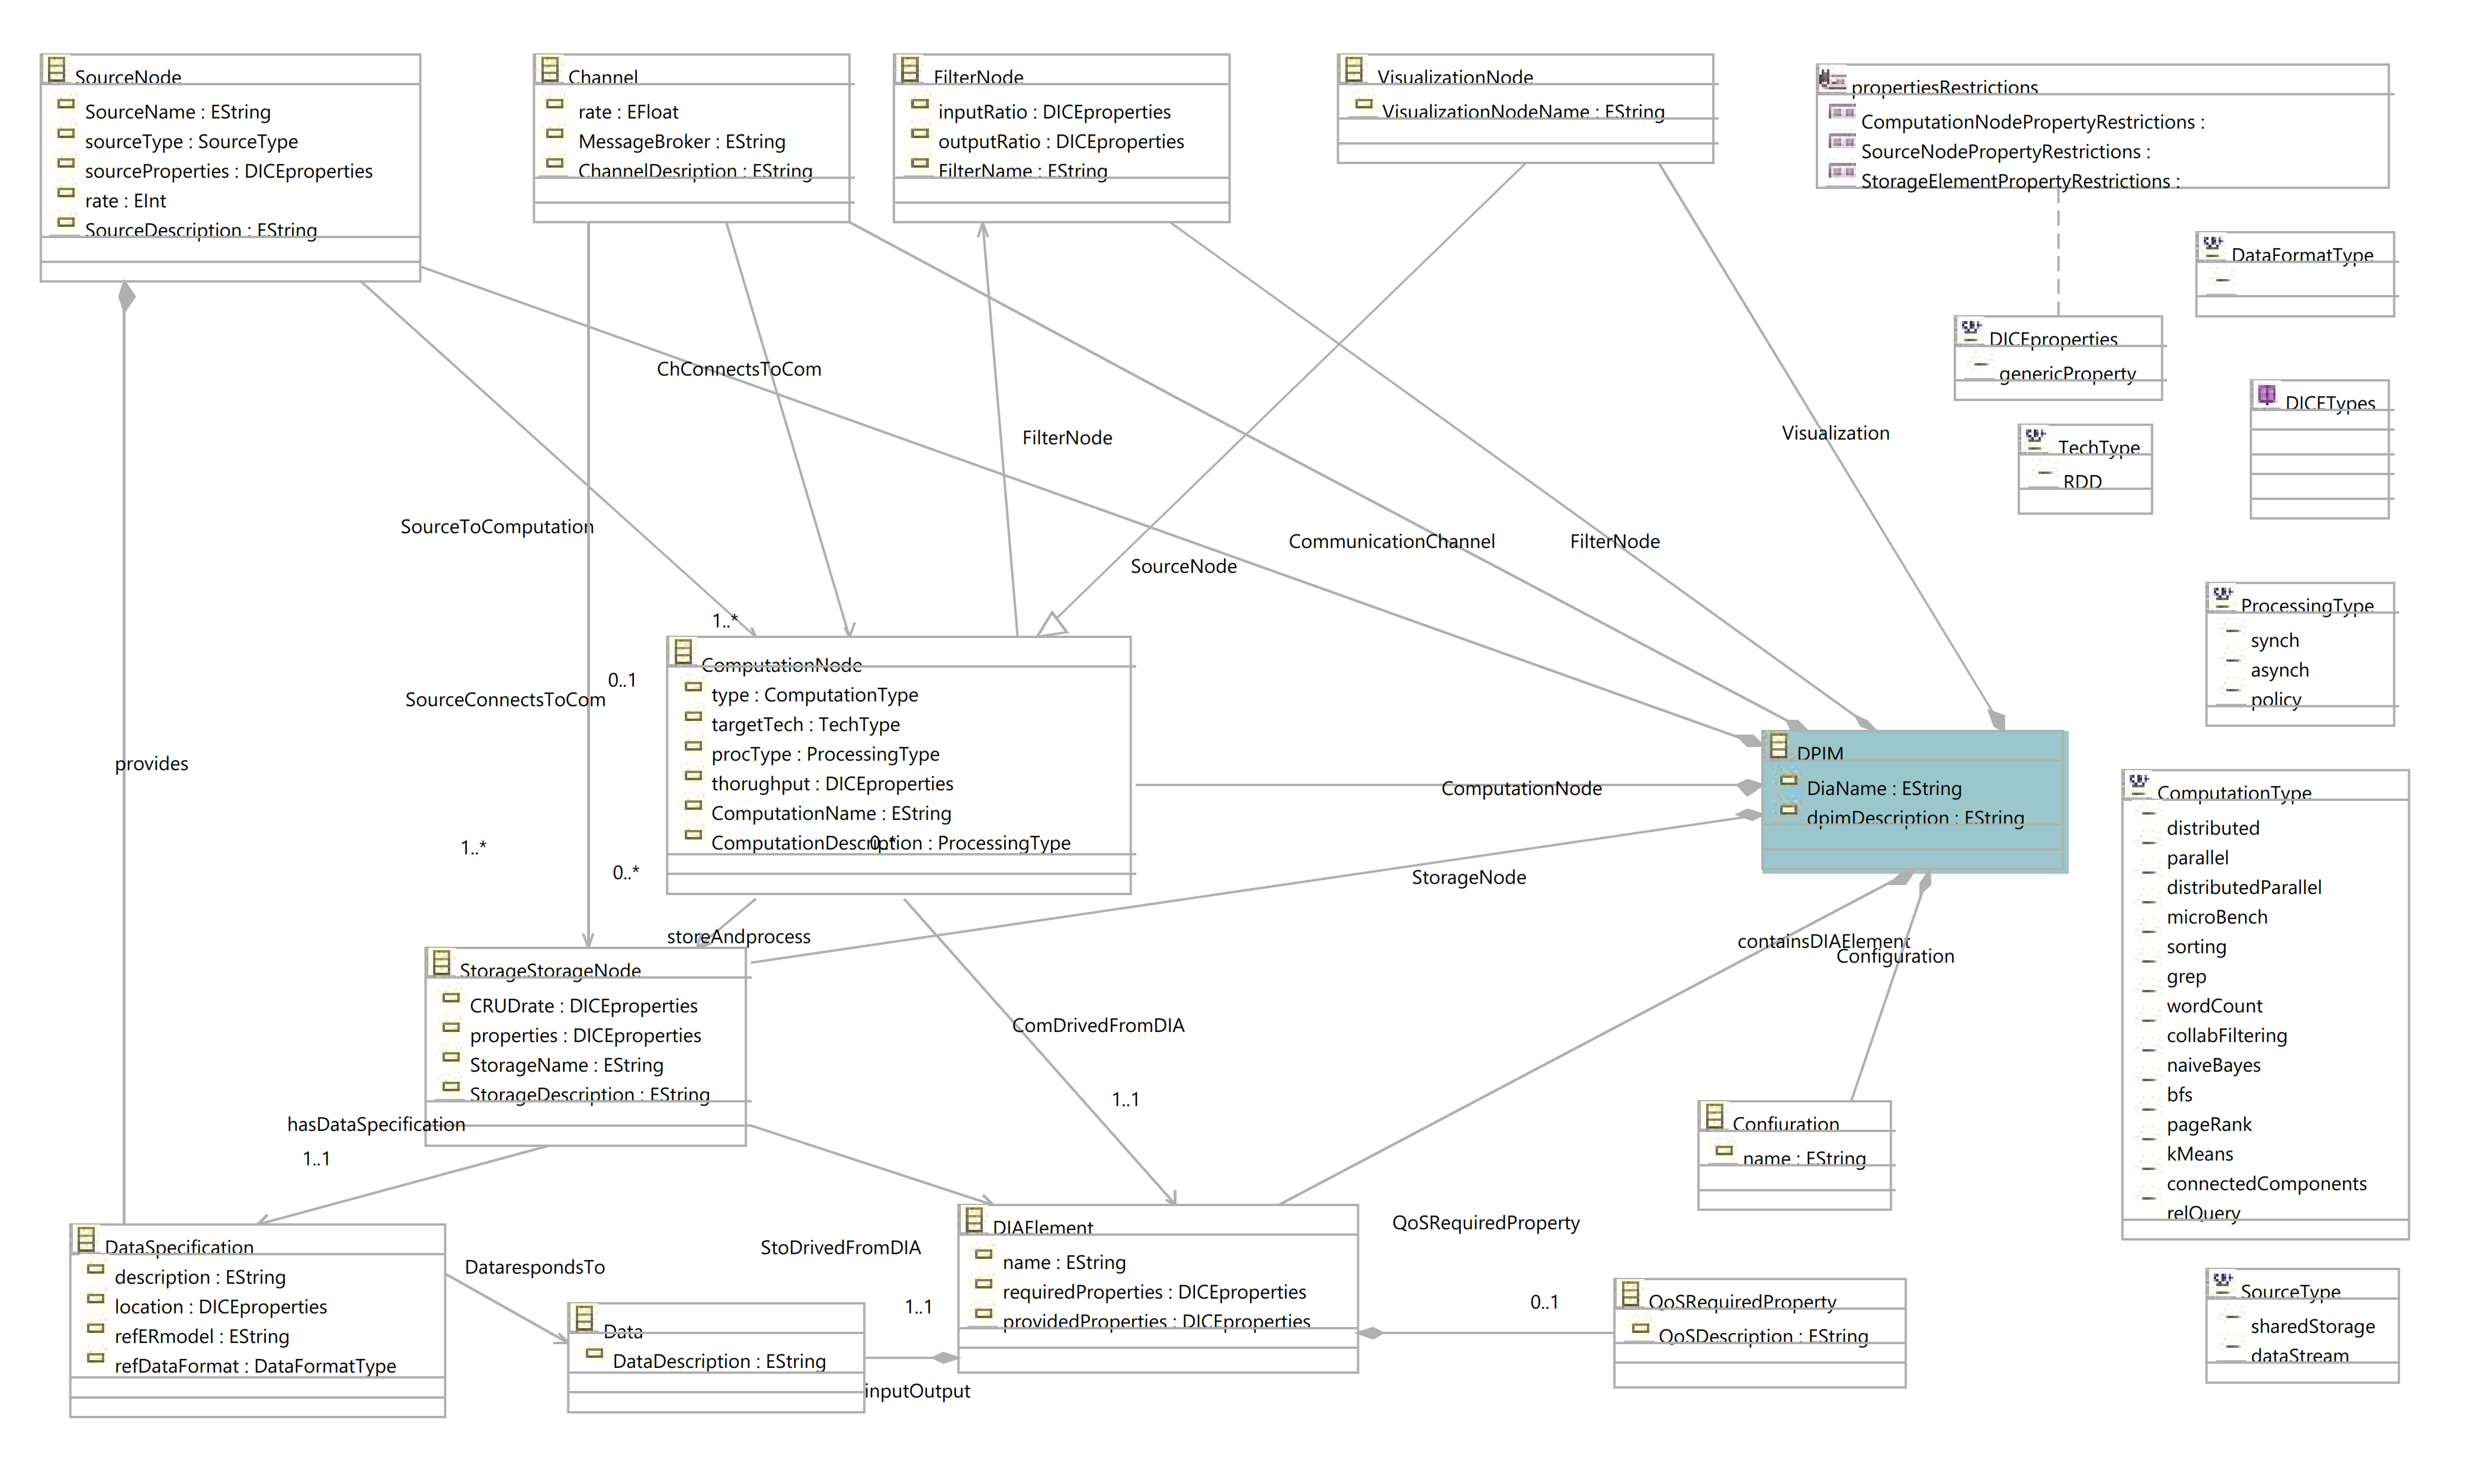
\includegraphics[width=\textwidth]{Images/11.png}
\caption{\label{fig:metamodel}DICE DPIM metamodel.}
\end{sidewaysfigure}

\begin{figure}
\centering
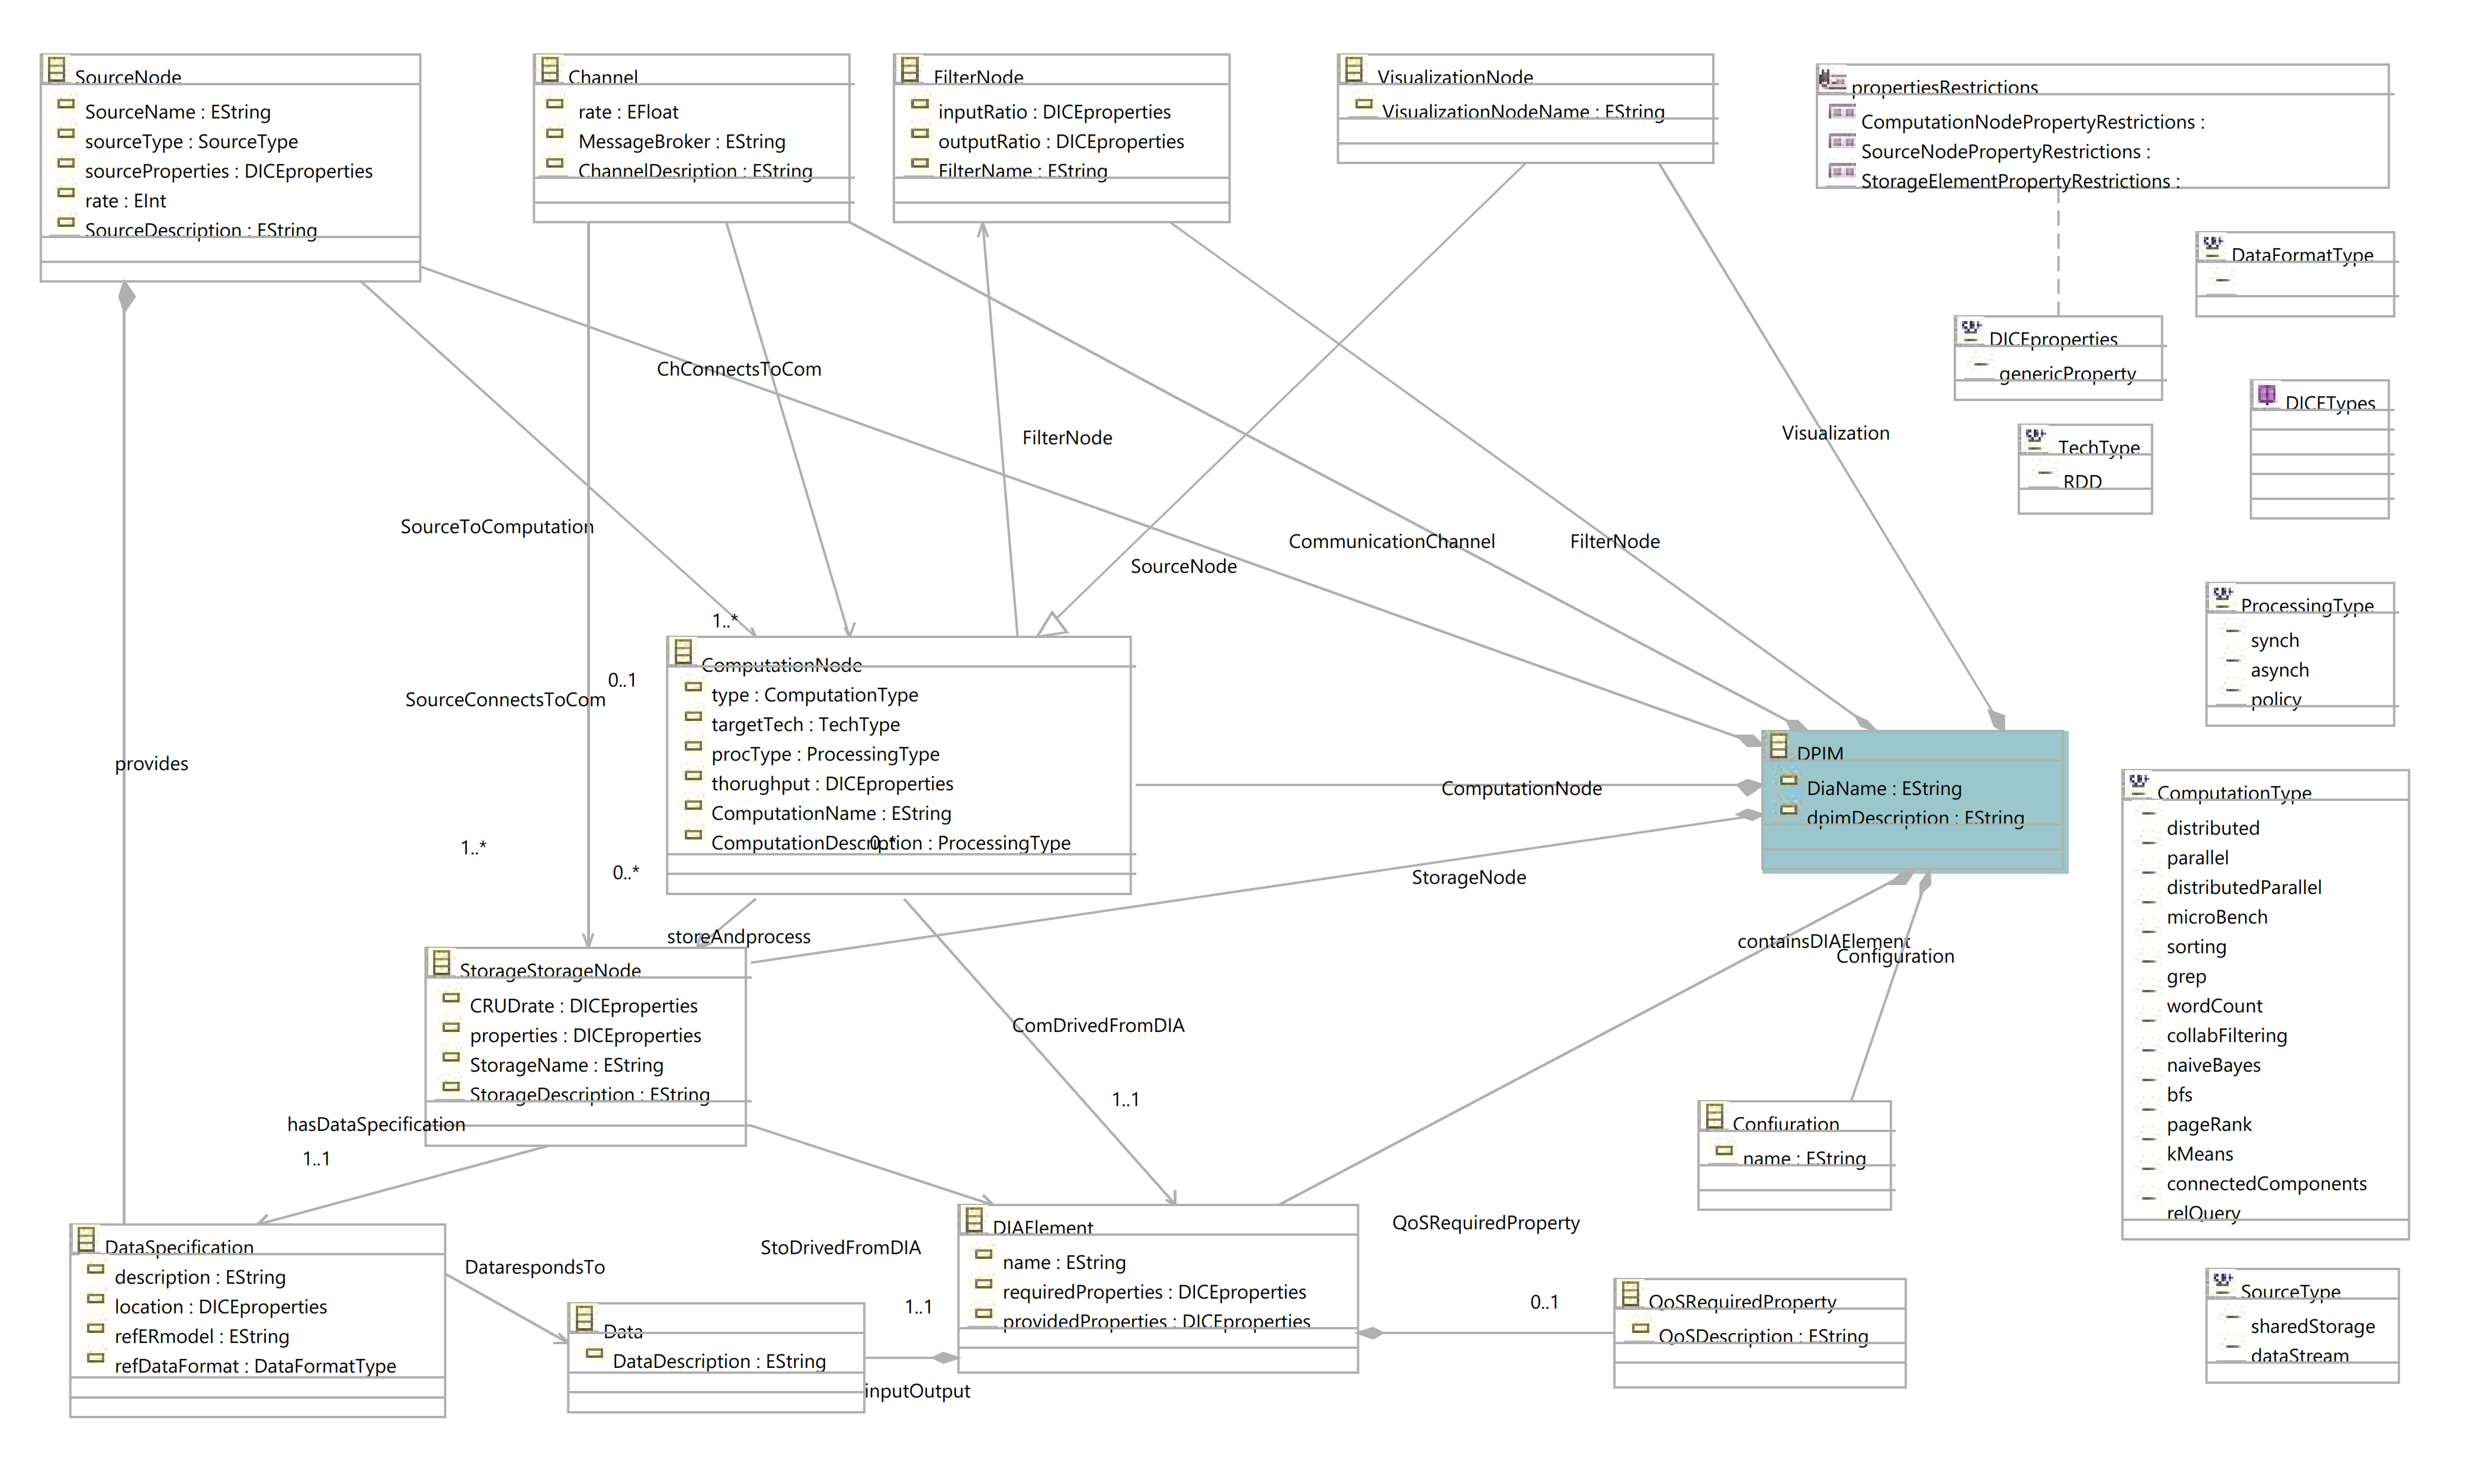
\includegraphics[width=\textwidth]{Images/11.png}
\caption{\label{fig:metamodel2}DICE DPIM metamodel in portrait form.}
\end{figure}

Here is the command to refer to another element (section, figure, table, ...) in the document: \emph{As discussed in Section~\ref{sect:overview} and as shown in Figure~\ref{fig:metamodel}, ...}. Here is how to introduce a bibliographic citation~\cite{DAM}. Bibliographic references should be included in a \texttt{.bib} file. 

Table generation is a bit complicated in Latex. You will soon become proficient, but to start you can rely on tools or external services. See for instance this \href{https://www.tablesgenerator.com}{https://www.tablesgenerator.com}. 

\subsection{Product perspective}

\subsection{Product functions}

\subsubsection{User Data Acquisition}
\subsubsection{User Data Retrieval}
\subsubsection{Health Emergency Monitoring}
\subsubsection{Run Events Management}

\subsection{User characteristics}
\subsubsection{Actors}
\begin{itemize}
\item Data4Help User
\item Third Party
\item Data Source Application
\item Ambulance system
\item Run organizer
\item Run spectator
\item Runner
\item Sys Admin
\end{itemize}
\subsection{Assumptions, dependencies and constraints}
\subsubsection{Domain Assumptions}
\subsubsection{Software dependencies}
Software dependencies: Maps, ambulance API
\subsubsection{Hardware constraints}
Server(?), Smartphone/Smartwear/smartdevices, GPS, 4G, sensors

%------------------------------------------------------------------------------------------------------------------------------------------------
\clearpage
{\color{Blue}{\section{Specific Requirements}}}
\label{sect:requirements}
Organize this section according to the rules defined in the project description. 
\subsection{External Interface Requirements}
\subsubsection{User Interface}
\subsubsection{Hardware Interfaces}
\subsubsection{Software Interfaces}
\subsubsection{Communication Interfaces}
\subsection{Functional Requirements}
\subsection{Scenarios}
\subsubsection{Scenario 1}
While talking, John tells his friend Matt about a new service called Data4Help that helps you keeping track of your health status. Frank, interested in checking his heart rate, downloads the app on his smartphone and fires it up. The app asks him to register to the service by filling a form with his personal information, including his fiscal code and a password of his choice that will be used as credentials for the login. 
After filling the form he clicks on the final checkbox to accept the personal data treatment policy.
Right after clicking on the "Submit" button, Frank receives a notification saying he successfully registered to Data4Help.
\subsubsection{Scenario 2}
Mary, a Data4Help customer, received for her birthday the new Eppol iClock. After the initial setting of the device, she decides to download the Data4Help application for her smartwatch. Once installed, she logs in with her accountand right after that, the "Device Management"
%secondo me meglio un home page qui
 view of the application appears. Mary taps on the iClock icon and by selecting "Heart Rate" from a dropdown she assigns the tracking of that paramater to her smartwatch. With the same procedure, she assigns to her smartphone the tracking of the "Position" parameter.
Finally, she clicks on the "Confirm" button and the app saves the settings and returns back to the home page.
\subsubsection{Scenario 3}
Steve, a Data4Help customer with diabete, needs to periodically check the glucose levels observed by his medical device connected with the Data4Help application on his smartphone. For doing this, he starts the Data4Help application and when the homepage shows up he  clicks on the "myData" tab. A nice view appears, containing all the information about his monitored health parameters with a lot of colorful diagrams. Steve f ilters out the displayed content by selecting the "Glucose Level" radio button on the top of the page and he changes the information granularity from "Week" to "Day" using a dropdown.  
\subsubsection{Scenario 4}
Michael Garcia, Boyer Pharmaceutical CEO, heard about the Data4Help service and in agreement with the Administrative Board, he decided to introduce it in the company. He visits  www.trackme.com/data4help and clicks on the "Business Solutions" section in order to register his company as a registered third party of the service. Tp do this, Michael fills in the registration form with all the requested information about the company, including the VAT-number, an e-mail and a password. After that he clicks on the "Submit" button and he immediately receives an e-mail with a link to complete the registration procedure.
\subsubsection{Scenario 5}
Brian, patient of the Lenox Private Medical Center, was released  yesterday. The clinic, registered to the Data4Help service, decides to monitor his health status to see if the treatment he was under reached the desired results.
The doctor that was in charge of Brian logs in to the Data4Help reserved page of the clinic. Once logged in, he inserts Brian's fiscal code and selects from a checkbox "Heart Beat" and "Temperature" as the data to monitor. Finally he chooses from a dropdown "3 months" as the observation period.
As soon as the doctor clicks on the "Send Request" button on the bottom of the page, Brian receives a notification on his smartphone. He launches the application and when the home page shows up he taps on the "Incoming Requests" tab. Here he sees the request coming from Lenox Private Medical Center. He briefly reads the description and he clicks on the "Accept" button. A confirmation e-mail, saying the patient accepted the treatment of his personal data, is immediately sent to Lenox Private Medical Center.
The doctor sees the e-mail and goes in the "Sent Requests" section of the Data4Help personal page of the company. After clicking on Brian's answer, all the requested data are displayed on screen.
\subsubsection{Scenario 6}
Pfuzer, a big pharmaceutical company registered to Data4Help service, needs to gather the heart rate data of all the italian young people under 30 years old for a market analysis aimed at evaluating the production of a new drug against heart disease. For this reason Todd Chavez, the marketing manager of the company, goes to the Pfuzer personal Data4Help page and once logged  in he clicks on the "Aggregated requests" tab in the home page. Once in the page he types in the textbox "Italy" as location, and selects the age range "<= 30" using a slider. Then he clicks on "Send request" on the bottom of the page and a warning message is immediately displayed on screen saying that the request cannot be satisfied. For this reason, Todd decides to untighten the search parameters. After changing them the constraints are satisfied and the requested data is immediately displayed on screen.
\subsubsection{Scenario 7}
Andrew decided to buy the new iClock as a gift for the birthday of his grandfather Leonard, 93 years old, who suffers from severe heart problems and lives alone. Since Leonard would like to be autonomous, his new device with AuotmatedSOS service active on it, grants him a safer life.

One night Leonard wakes up with severe chest pains. The iClock immediately detects the "heart rate" parameter exceeded the maximum threshold and shows a noisy emergency alert, saying that an ambulance will be called if the user doesn't abort in the following minute. Leonard is really sick and is not able to abort the operation. In few minutes an ambulance arrives and Leonard is immediately rescued.
\subsubsection{Scenario 8}
William suffers from epilepsy. The attacks are not very frequent but they are so strong that a few months ago he fell and he got a nasty head injury. While looking for an automated solution to check on his conditions, he hears about AutomatedSOS and decides to activate the service provided by Data4Help.

At first he sets the threshold of the tracked parameters with the help of his doctor and he adds the contacts of his parents. When the wristwatch detects repetitive shaking motion, it automatically sends the user’s bluetooth-connected phone text and call alerts to the designated recipients. Within seconds, family members receive these alerts, which include the date, time and GPS location of the event.
\subsubsection{Scenario 9}
\subsubsection{Scenario 10}
\subsection{Use Case}
\begin{table}[]
\begin{tabular}{|l|p{12cm}|}
\hline
Name             & User registration \\ \hline
Actor            & User \\ \hline
Entry conditions & App installed on user's device (and run while not logged in?) \\ \hline
Events flow      & \begin{enumerate}
\item Click on the "Subscribe" button
\item Fill the registration form and the account credentials
\item Accept the terms of service and the privacy policy
\item Click on the "Submit" button
\item The system elaborate the registration and send back a notification
\end{enumerate} 
\\ \hline
Exit conditions  & Registration is successful and the user is informed via notification \\ \hline
Exceptions       & \begin{enumerate}
\item The user is already registered
\item There is some invalid data in the form
\item The email is already used
\item Terms of service or Privacy policy haven't been checked
\end{enumerate} All the exceptions take the user back to the registration procedure \\ \hline
\end{tabular}
\end{table}

\begin{table}[]
\begin{tabular}{|l|p{12cm}|}
\hline
Name             & User log in \\ \hline
Actor            & User \\ \hline
Entry conditions & App installed on user's device and user already registered to Data4Help \\ \hline
Events flow      & \begin{enumerate}
\item Click on the "Log in" button
\item The user enter his/her credentials
\item Click on the "Enter" button
\item The log in was successful and the user is redirected to the home page of the App
\end{enumerate} \\ \hline
Exit conditions  & The log in is successful and the user is redirected to home page \\ \hline
Exceptions       & \begin{enumerate}
\item Credentials aren't valid
\end{enumerate} The exceptions are notified to the user and the Log in procedure restart \\ \hline
\end{tabular}
\end{table}

\begin{table}[]
\begin{tabular}{|l|p{12cm}|}
\hline
Name             & Device Management \\ \hline
Actor            & User \\ \hline
Entry conditions & User enter in the "Device Management" pannel of the App \\ \hline
Events flow      & \begin{enumerate}
\item The list of devices connected to the account is shown
\item The user select which device to configure
\item For that device, the list of all the possible parameter that it can track is shown
\item The user turn On/Off the tracking of each parameter
\item Click on the "Confirm" button
\end{enumerate} \\ \hline
Exit conditions  & The user have set his/her preference and saves them \\ \hline
Exceptions       & \begin{enumerate}
\item the parameter is already tracked from a more reliable source (maybe??)
\end{enumerate} \\ \hline
\end{tabular}
\end{table}

\begin{table}[]
\begin{tabular}{|l|p{12cm}|}
\hline
Name             & MyData \\ \hline
Actor            & User \\ \hline
Entry conditions & User enter in the "MyData" tab of the app \\ \hline
Events flow      & \begin{enumerate}
\item The system shows all the user gathered info
\item A top bar is presented to the user to filter the search
\item Whenever a filer is changed the app respond with the filtered information
\end{enumerate} \\ \hline
Exit conditions  & The user exit the information tab \\ \hline
Exceptions       & \begin{enumerate}
\item the system haven't gathered any info yet
\end{enumerate} The exceptions are notified to the user and the MyData page is shown with the available data \\ \hline
\end{tabular}
\end{table}

\begin{table}[]
\begin{tabular}{|l|p{12cm}|}
\hline
Name             & Third Party Registration \\ \hline
Actor            & Third Party \\ \hline
Entry conditions & The third party clicks on "Business Solutions" on www.trackme.com/data4help \\ \hline
Events flow      & \begin{enumerate}
\item Click on the "Register" button
\item Fill the form with information regarding the company
\item Click on the "Submit" button
\end{enumerate} \\ \hline
Exit conditions  & Registration is completed and a notification is sent via e-mail \\ \hline
Exceptions       & \begin{enumerate}
\item Company already registered
\item email already in use
\end{enumerate} All the exceptions are notified and the procedure goes back to registration \\ \hline
\end{tabular}
\end{table}

\begin{table}[]
\begin{tabular}{|l|p{12cm}|}
\hline
Name             & Third Party Log in \\ \hline
Actor            & Third Party \\ \hline
Entry conditions & The third party goes on www.trackme.com/data4help and click "Log in" \\ \hline
Events flow      & \begin{enumerate}
\item Click on the "Log in" button
\item Enter the company credentials
\item Click on the "Enter" button
\end{enumerate} \\ \hline
Exit conditions  & Log in is successful and the client is redirected to its reserved page  \\ \hline
Exceptions       & \begin{enumerate}
\item Credentials aren't valid
\end{enumerate} The exceptions are notified to the client and the Log in procedure restart  \\ \hline
\end{tabular}
\end{table}

\begin{table}[]
\begin{tabular}{|l|p{12cm}|}
\hline
Name             & Single Data Request \\ \hline
Actor            & Third Party, User \\ \hline
Entry conditions & A third party client is logged in and goes under "Single Data Request"  \\ \hline
Events flow      & \begin{enumerate}
\item Click on "Single Data Request"
\item Insert the fiscal code of the person whose data are requested
\item Check which data to monitor form a checklist
\item Select the observation period
\item Click on "Send" button
\item The request is notified to the user
\item The user logs into the App and goes under "Incoming Request"
\item The user select whether or not to accept the request
\item The result is notified via e-mail to the third party
\item If the user accepted, the information are made available under the "Sent Request" section of the Data4Help personal page of the company
\end{enumerate} \\ \hline
Exit conditions  & The user has responded to the request and, if successful, the data are made available to the third company \\ \hline
Exceptions       & \begin{itemize}
\item The observation period covers a time period in the future
\end{itemize} This exception launches the subscription procedure
\begin{enumerate}
\item The user refuse the request
\end{enumerate} This exception is notified to the third party and the request ends\\  \hline
\end{tabular}
\end{table}

\begin{table}[]
\begin{tabular}{|l|p{12cm}|}
\hline
Name             & Aggregate Data Request \\ \hline
Actor            & Third Party, Data4Help (maybe?) \\ \hline
Entry conditions & A ttesthird party client is logged in and goes under "Aggregate Data Request" \\ \hline
Events flow      & \begin{enumerate}
\item Click on "Aggregate Data Request"
\item Insert the location of the data
\item Select the age range
\item Customize any other filter on the data
\item Click the "Send request" button
\item The request is elaborated throught the Anonym? procedure
\item On request successful, the data are made available uder the "Sent Request" section of the Data4Help personal page of the company
\end{enumerate} \\ \hline
Exit conditions  & The request was successful and the data are made available to the third company \\ \hline
Exceptions       & \begin{itemize}
\item An observation period is selected and it covers a time period in the future
\end{itemize} This exception launches the subscription procedure
\begin{enumerate}
\item Anonym? returns request rejected due to lack of anonymity
\end{enumerate} The exception notifies the third party on reasons of the rejection and returns to the Aggregate Data Request page\\ \hline
\end{tabular}
\end{table}

\begin{table}[]
\begin{tabular}{|l|p{12cm}|}
\hline
Name             & Data Subscription \\ \hline
Actor            & Third party \\ \hline
Entry conditions & A request, for single or aggregate data, has been made with an observation period that extend in the future \\ \hline
Events flow      & \begin{enumerate}
\item If the request is successful, the third company is updated about the changes in the data that it requested
\end{enumerate} \\ \hline
Exit conditions  & The observation period elapses and the subscription end \\ \hline
Exceptions       & \begin{enumerate}
\item Data aren't available anymore
\end{enumerate} The exception are notified to the client via e-mail \\ \hline
\end{tabular}
\end{table}

\begin{table}[]
\begin{tabular}{|l|p{12cm}|}
\hline
Name             & Anonym? \\ \hline
Actor            & Data4Help \\ \hline
Entry conditions & Data4Help recives a request for aggregate data and the system algorithm anonymize the data \\ \hline
Events flow      & \begin{enumerate}
\item An aggregate request arrives at Data4Help
\item The anonymization algorithm launches on the available data
\item It return the anonymized data to be seen by the third party
\end{enumerate} \\ \hline
Exit conditions  & The data were successfully anonymized by the algorithm \\ \hline
Exceptions       & \begin{enumerate}
\item The available data are scarce ($<=$1000) hence the anonymization is impossible
\end{enumerate} This exception notifies the third party that its request has been rejected\\ \hline
\end{tabular}
\end{table}

\begin{table}[]
\begin{tabular}{|l|p{12cm}|}
\hline
Name             & AutomatedSOS Subscription \\ \hline
Actor            & User, AutomatedSOS \\ \hline
Entry conditions & User enters in the "AutomatedSOS" pannel under the App \\ \hline
Events flow      & \begin{enumerate}
\item Click on "Subscribe"
\item Configure the settings
\item Accept clauses
\item Start Supervisor
\end{enumerate} \\ \hline
Exit conditions  & The user has subscribed to the service and the Supervisor starts \\ \hline
Exceptions       & \begin{enumerate}
\item User cannot access to the service due to lack of devices that can track his/her real time status
\end{enumerate} The exceptions are notified to the client that is brought back to the AutomatedSOS panel\\ \hline
\end{tabular}
\end{table}

\begin{table}[]
\begin{tabular}{|l|p{12cm}|}
\hline
Name             & Supervisor \\ \hline
Actor            & AutomatedSOS, User, Third party (emergency) \\ \hline
Entry conditions & The user has subscribed successfully to the AutomatedSOS service and his/her supervisor has started \\ \hline
Events flow      & \begin{enumerate}
\item Monitor real time data
\item Check for threshold constraint
\item Repeat
\end{enumerate} \\ \hline
Exit conditions  & User unsubscribe from the AutomatedSOS service \\ \hline
Exceptions       & \begin{itemize}
\item Some parameter went over its threshold
\end{itemize} This exception notifies the client and AutometedSOS system proceed to call emergency numbers \begin{enumerate}
\item Lost device for data acquisition
\end{enumerate} This exception notifies the client and pause the Supervisor until the problem is fixed \\ \hline
\end{tabular}
\end{table}

\begin{table}[]
\begin{tabular}{|l|p{12cm}|}
\hline
Name             & Run enroll \\ \hline
Actor            & User, Track4Run \\ \hline
Entry conditions & User enters in the "Enroll" panel, under the "Track4Run" tab in the App  \\ \hline
Events flow      & \begin{enumerate}
\item Choose from a list to which run to enroll
\item Click on the "Enroll" button
\item Accept the clauses
\item Process the enrollment and start the Tracker
\end{enumerate} \\ \hline
Exit conditions  & The user has successfully enrolled to the run and the Tracker started running \\ \hline
Exceptions       & \begin{enumerate}
\item The user doen't possess a device able to Track the runner
\item The user is in a bad shape for a run, medical advice is suggested
\end{enumerate} This exceptions is notified to the client and the procedure goes on\\ \hline
\end{tabular}
\end{table}

\begin{table}[]
\begin{tabular}{|l|p{12cm}|}
\hline
Name             & Tracker \\ \hline
Actor            & Track4Run, User,  \\ \hline
Entry conditions & The user has enrolled for a run \\ \hline
Events flow      & \begin{enumerate}
\item Stay on idle till starts of the run
\item On wake up, keep track of real time location of the user
\end{enumerate} \\ \hline
Exit conditions  & The run ends and the Tracker leave the user \\ \hline
Exceptions       & \begin{enumerate}
\item Lost device for real time location
\end{enumerate} This exception is notified to the client and the procedure goes on
\begin{enumerate}
\item User unsubscribe form the Run
\end{enumerate} This exception kills the Tracker and remove the user from the run\\ \hline
\end{tabular}
\end{table}

\begin{table}[]
\begin{tabular}{|l|p{12cm}|}
\hline
Name             & Run "unsubscription" \\ \hline
Actor            & User, Track4Run \\ \hline
Entry conditions & User already enrolled on a Run and he/she want to unsubscribe \\ \hline
Events flow      & \begin{enumerate}
\item Look up under "Your Runs" tab for the desired run
\item Click on the "Unsubscribe" button
\item Notifies the Tracker
\end{enumerate} \\ \hline
Exit conditions  & User has successfully unsubscribed from the run \\ \hline
Exceptions       & ? \\ \hline
\end{tabular}
\end{table}

\begin{table}[]
\begin{tabular}{|l|p{12cm}|}
\hline
Name             & Watch Run \\ \hline
Actor            & User (Spectator), Track4Run, Users (Runners) \\ \hline
Entry conditions & A spectator goes under the "Live" section of Track4Run and select an ongoing run \\ \hline
Events flow      & \begin{enumerate}
\item Select a Run form the list of ongoing runs
\item Enter information about the desired runner
\item Watch the map of the run with the real time GPS tracking of the searched runner
\end{enumerate} \\ \hline
Exit conditions  & Run ends or spectator exit from the live page \\ \hline
Exceptions       & \begin{enumerate}
\item Runner has connection problems
\item Spectator has connection problems
\item Server has connection problems
\end{enumerate} All exception are notified to the spectator and the process goes on\\ \hline
\end{tabular}
\end{table}

\begin{table}[]
\begin{tabular}{|l|p{12cm}|}
\hline
Name             & Create a Run \\ \hline
Actor            & User (Organizer), Track4Run \\ \hline
Entry conditions & The organizer goes under the "Create Run" panel of the Track4Run section of the App \\ \hline
Events flow      & \begin{enumerate}
\item Click on the "Create Run" button
\item Enter information about the run
\item Select the run path from the map
\item Click on the "Create" button
\end{enumerate} \\ \hline
Exit conditions  & The organizer has successfully created a run \\ \hline
Exceptions       & ?\\ \hline
\end{tabular}
\end{table}

\begin{table}[]
\begin{tabular}{|l|p{12cm}|}
\hline
Name             & Run modification/cancellation \\ \hline
Actor            & User (Organizer), Track4Run \\ \hline
Entry conditions & The organizer goes under the "Your Run" panel of the Track4Run section of the App \\ \hline
Events flow      & \begin{enumerate}
\item Select the run you want to modify
\item Modify the information of the run
\item Modify the path of the run from the map
\item Select whether to cancel or not the run
\item Click on the "Confirm" button
\end{enumerate} \\ \hline
Exit conditions  & The organizer has successfully modified or canceled the run \\ \hline
Exceptions       & On success, notifies all the partecipants about the changes\\ \hline
\end{tabular}
\end{table}

\subsection{Performance Requirements}
\subsection{Design Constraints}
\subsubsection{Standard compliance}
\subsubsection{Hardware limitations}
\subsubsection{Any other constraint}
\subsection{Software System Attributes}
\subsubsection{Reliability}
\subsubsection{Availability}
\subsubsection{Security}
\subsubsection{Maintainability}
\subsubsection{Portability}


%------------------------------------------------------------------------------------------------------------------------------------------------
\clearpage
{\color{Blue}{\section{Formal Analysis Using Alloy}}}
\label{sect:alloy}
Organize this section according to the rules defined in the project description. 


%------------------------------------------------------------------------------------------------------------------------------------------------
\clearpage
{\color{Blue}{\section{Effort Spent}}}
\label{sect:effort}
Provide here information about how much effort each group member spent in working at this document. We would appreciate details here.




\end{document}